\chapter{归纳不变式自动生成工具的设计}\label{chap:design}

本章节将介绍rlTLA的具体设计,每个模块的职责和功能。

总体上,工具需要完成一下工作:
\begin{itemize}
    \item 解析用户输入,存储预备后续使用;
    \item 检验模块预先生成用于检测三个属性的配置文件(.cfg)。对生成模块所生成的候选不变式检验其正确性、独立性和与已有不变式析取结果的递归性,
    生成归纳反例,回传给生成模块;
    \item 生成模块,基于用户输入和检验模块的结果,生成合适的不变式;
    \item 其他非功能模块,包括日志模块,计时模块等;
\end{itemize}

rlTLA的工作流如图\ref{fig:rltla}所示,功能模块主要分为候选不变式生成模块(Invariant Generator),候选不变式检验模块(TLC/Apalache)两个部分。
其中候选不变式生成模块接入了强化学习,训练强化模型智能体,以提高候选不变式的生成效率和准确率。
候选不变式检验模块则接入了TLC或Apalache,对生成的候选不变式进行验证,检验其正确性,独立性和与已有不变式析取结果的递归性,并将结果返回给生成模块。
在初始化阶段,候选不变式检验模块还需要生成用于检测这三种属性的配置文件(.cfg),并生成初始的归纳反例。
目前系统接受 endive 提供的数据源,使用 endive 中的对规约人工标记的谓词,作为生成候选不变式的种子(seed)。
系统的输出是对一系列引理不变式的析取范式,对于系统而言,是一个包含 $Safe$ 属性的归纳不变式。

基本的逻辑结构如伪代码\ref{alg:rltla-workflow}展示。
初始化时候,候选的归纳不变式首先析取$Safe$属性,然后生成候选不变式的CTI(Counterexample to Induction)。
在每一轮的迭代中,强化学习系统都会不断地生成一个个候选不变子式,直到生成的子式在系统运行环境中是不变式,且不会被已有的不变式所包含。
这样的不变式便会加入到候选的归纳不变式中做析取,直到对候选归纳不变式生成的CTI为空,即不再有反例产生。
这说明现在系统中所有不变式的析取结果是一个包含$Safe$属性归纳不变式,也就是得到了归纳不变式,系统选择将这个结果输出给用户。


\begin{figure}
    \centering
    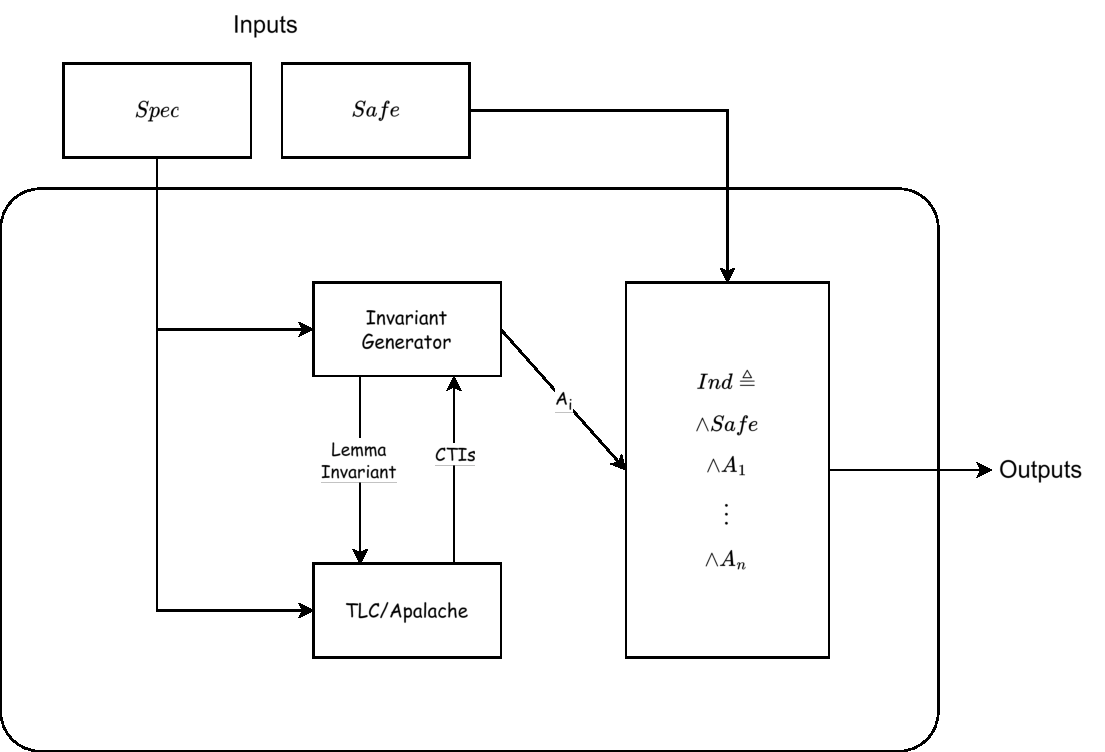
\includegraphics[width=0.7\textwidth]{figures/workflow.pdf}
    \caption{rlTLA-workflow}
    \label{fig:rltla}
\end{figure}

\begin{algorithm}
    \caption[short]{workflow of rlTLA}
    \label{alg:rltla-workflow}
    
    \begin{algorithmic}[1]
        \REQUIRE \ \\
        $M$: Finite instance of parameterized system\\
        $Safe$: Safety property
		\ENSURE \ \\
        $Ind$: Inductive Invariant Candidiate
		\STATE $Ind \gets Safe$
        \STATE $IndCTIs \gets GenrateIndCTIs(M, Ind)$
        \WHILE{$IndCTIs$ is not empty}
            \STATE $InvCTIs \gets IndCTIs$
            \WHILE{True}
                \STATE $Inv \gets GenerateCandidateInvariant(M, IndCTIs)$
                \STATE $InvCTIs \gets GenrateInvCTIs(M, Inv)$
                \IF{$InvCTIs$ is not empty}
                    \STATE $Continue$
                \ENDIF
                \IF {not $CheckDerivation(Ind, Inv)$} 
                    \STATE $Ind = Ind \wedge Inv$
                    \STATE $Break$
                \ENDIF
            \ENDWHILE
            \STATE $IndCTIs \gets GenrateIndCTIs(M, Ind)$
        \ENDWHILE
        \RETURN $Ind$
    \end{algorithmic}
\end{algorithm}

\section{候选不变式生成模块}

对于一个给定的规约的有限大小的实例,候选不变式生成模块的工具就是生成一系列在规约的每个状态下都成立的候选不变式,这些不变式以一阶逻辑谓词的形式存在。
为了找到这些不变式,我们使用一种基于语法合成指导的归纳不变式生成技术。
我们从输入的种子(seed)谓词中,按照强化学习模块的意愿选择一部分种子谓词,并按照语法组合成一个可能的不变式。
每个种子谓词都是针对系统状态变量的布尔表达式。
当然,我们也有可能采取给出种子谓词的否定,根据\TLA 的语法,我们只需要在给出的谓词前面加上否定符号 \textbf{“\~{}”}即可。
这部分的决定权交给强化学习模块,强化学习模块会根据当前的状态,选择一个合适的种子谓词,或者它的否定。

一个不变式的语法大致可以表达为:
\begin{align}
    <lemma> &: = <quant>:<expr>   \\
    <quant> &:= \forall x\ \backslash in\ SetA | \exists y\ \backslash in\ SetB \\
    <expr>  &:= <seed>| \sim<seed> | <seed> \wedge <seed>
\end{align}
注意到本文中所提及的大部分的\TLA 规约都带有存在量词和全程量词,我们直接将这一部分量词当作输入的一部分。
尽管可以带来多余的量词表达式,但是这部分量词并不会对整个谓词的布尔值带来实际的影响,这部分多余的量词可以不做处理。
另外,我们对于引理不变式内部每个谓词之间的连接方式统一选择了合取符号“$\vee$”。
这是因为,一方面这种语法在表达归纳不变已经足够完备\cite{or-complete};
另一方面,由于简化了种子谓词之间的链接方式,也可以帮助了我们简化问题,缩小了搜索不变式的空间。


\section{强化学习在生成模块中的应用}

本文的目的是希望研究强化学习在自动的归纳不变式生成过程中的应用。
强化学习是一种通过智能体和环境的交互,智能体通过观察环境的状态,采取行动,获得奖励,来学习如何在环境中获取最大的奖励。
在本文中,强化学习被应用于生成归纳不变式的各个析取子式,也就是候选不变式。

强化学习模块接受\TLA 协议和检验模块对于本身生成的候选不变式的检验结果,修改策略,生成更加合理的候选不变式。
强化学习模块的输入是一个状态,输出是一个动作,动作是对于种子谓词的选择与否,和是否选择它的否定。

强化学习模块的目标是生成一个合适的候选不变式,这个候选不变式在规约的每个状态下都成立,且不会被已有的不变式的析取结果包含。
这个过程是自动化的,但人可以通过挑战对强化学习智能体在每个状态下的每个动作的选择给出合适的奖励或者惩罚,以指导智能体学习到
一个合适的策略,并应用到后续的候选不变式生成中。

最高的奖励应当给予给出最终的归纳不变式的行为,也就是给出了一个不变式,使得它和前面所有不变式的析取结果是归纳不变式的行为。
当强化学习模块给出一个不变式的时候,也应当给出一定的奖励。给出一个不变式,尤其是给出第一个不变式,往往是一个十分困难的过程。
而且,这一步也是实现最终目标的关键。因此,我们应当给予一定的奖励,以鼓励智能体继续学习。

生成一个已经被已有不变式包含的不变式,尽管没有意义,但也体现出智能体如何寻找不变式的能力,因此也应当给予一定的奖励。
这个奖励的值很小,但是也是必要的。因为这个过程是一个逐步的过程,智能体需要不断地尝试,才能找到一个合适的不变式。
但是,为了防止智能体的惰性,我们不允许智能体在已有的不变式上简单的合取上一个谓词,然后给出这个谓词作为候选不变式,
同样的,不允许在一个错误的不变式上去除掉一些谓词,以得到候选不变式。
这是简单的重复,是没有意义的,我们对智能体的这种行为应当给予惩罚。


\section{候选不变式检验模块}

候选不变式检验模块需要调用模型检查器,并且需要将输出解析,并将结果返回给生成模块。
对于候选不变式的检验,可以分为三个部分,分别是正确性、独立性和多个不变式析取结果的递归性。
引理\ref{con:inv_correct}表达了候选不变式的正确性,即候选不变式在规约的每个状态下都成立。
引理\ref{con:inv_indepence}表达了候选不变式的独立性,即新生成的候选不变式不能被已有的不变式的析取结果包含。
\begin{align}
    &Spec \triangleq Init \wedge [Next] \\
    &Spec \vDash Inv \label{con:inv_correct} \\
    &Spec \wedge IndCand \nvDash Inv \label{con:inv_indepence}
\end{align}

检验候选不变式的正确性,就是检验每个候选不变式是否在规约的每个状态下,布尔值都为真。
这个问题虽然简单,但是直觉上可能需要遍历许多状态和多个状态转移轨迹,可能需要很长的时间。
但是实际上,很多的不正确的候选不变式在规约的某个比较容易到达的状态被验证器检验出来,便可以退出了。
一个正确的不变式,尽管现在还不能成为归纳不变式,但是它确实我们需要归纳不变式的开始。

检验不变式的独立性时,我们需要验证新生成的候选不变式是否能被已有的不变式的析取结果包含。
检验不变式的独立性十分重要,尤其是对于指导强化学习生成候选不变式,
因为如果新生成的候选不变式能被已有的不变式的析取结果包含,那么生成模块为了得到更高的奖励,
会多生成这样的候选不变式,这样会导致不变式的重复,析取的结果的约束能力也不能加强,对状态空间不能做出有价值的修剪,
这样的不变式便是没有意义的。系统也就无法找到一个合适的归纳不变式。

检验归纳不变式的递归性,是我们工作的终点。
如果多个不变式的析取结果具有递归性,那么我们可以将这个析取结果作为归纳不变式,我们可以将这个结果输出,并结束这个循环。
对于不变式的递归性质,在引理\ref{con:init}和\ref{con:inductive}中已经提及。
归纳不变式需要包含所有的初始状态,并且,从归纳不变式约束的状态出发,进行状态转移,新生成的状态也需要满足归纳不变式。
另外,我们最根本的目的是证明安全属性,那么,归纳不变式需要蕴含安全属性。

